\documentclass[a4paper,12pt,english]{article}

\usepackage{amsmath}              % Math mode and text combined
\usepackage[english]{babel}       % Break words in the right place
\usepackage[style=apa]{biblatex}  % References
\usepackage[a4paper, margin={2.5cm}]{geometry} % Default A4 margins
\usepackage{graphicx}             % Images
\usepackage{subcaption}           % Composite images

\addbibresource{bibliography.bib}

\title{Securing Web-Based Electronic Elections
\\
\large Information Security Assignment - Group 1}

\author{Jarne Clauw
    \and
    Tibo De Peuter
    \and
    Robin Meersman
    \and
    Matthias Seghers
    \and
    Emma Vandewalle
    \and
    Tybo Verslype
}

\date{\today}

\begin{document}

\maketitle

\section{Introduction}\label{sec:introduction}

\section{Requirements for fair elections}\label{sec:requirements}

\cite{european-liberties-platform-2021}

\cite{cryptoeprint:2016/287}

More recently, there has been an increasing interest in online voting systems that are secure and trustworthy. (\cite{10.1145/2660267.2660315}, \cite{10.1007/978-3-030-51280-4_3}, \cite{263858}, \cite{halderman2015new}) Such systems 

\section{A design for secure web-based elections}\label{sec:design}

\begin{figure}
    \centering
    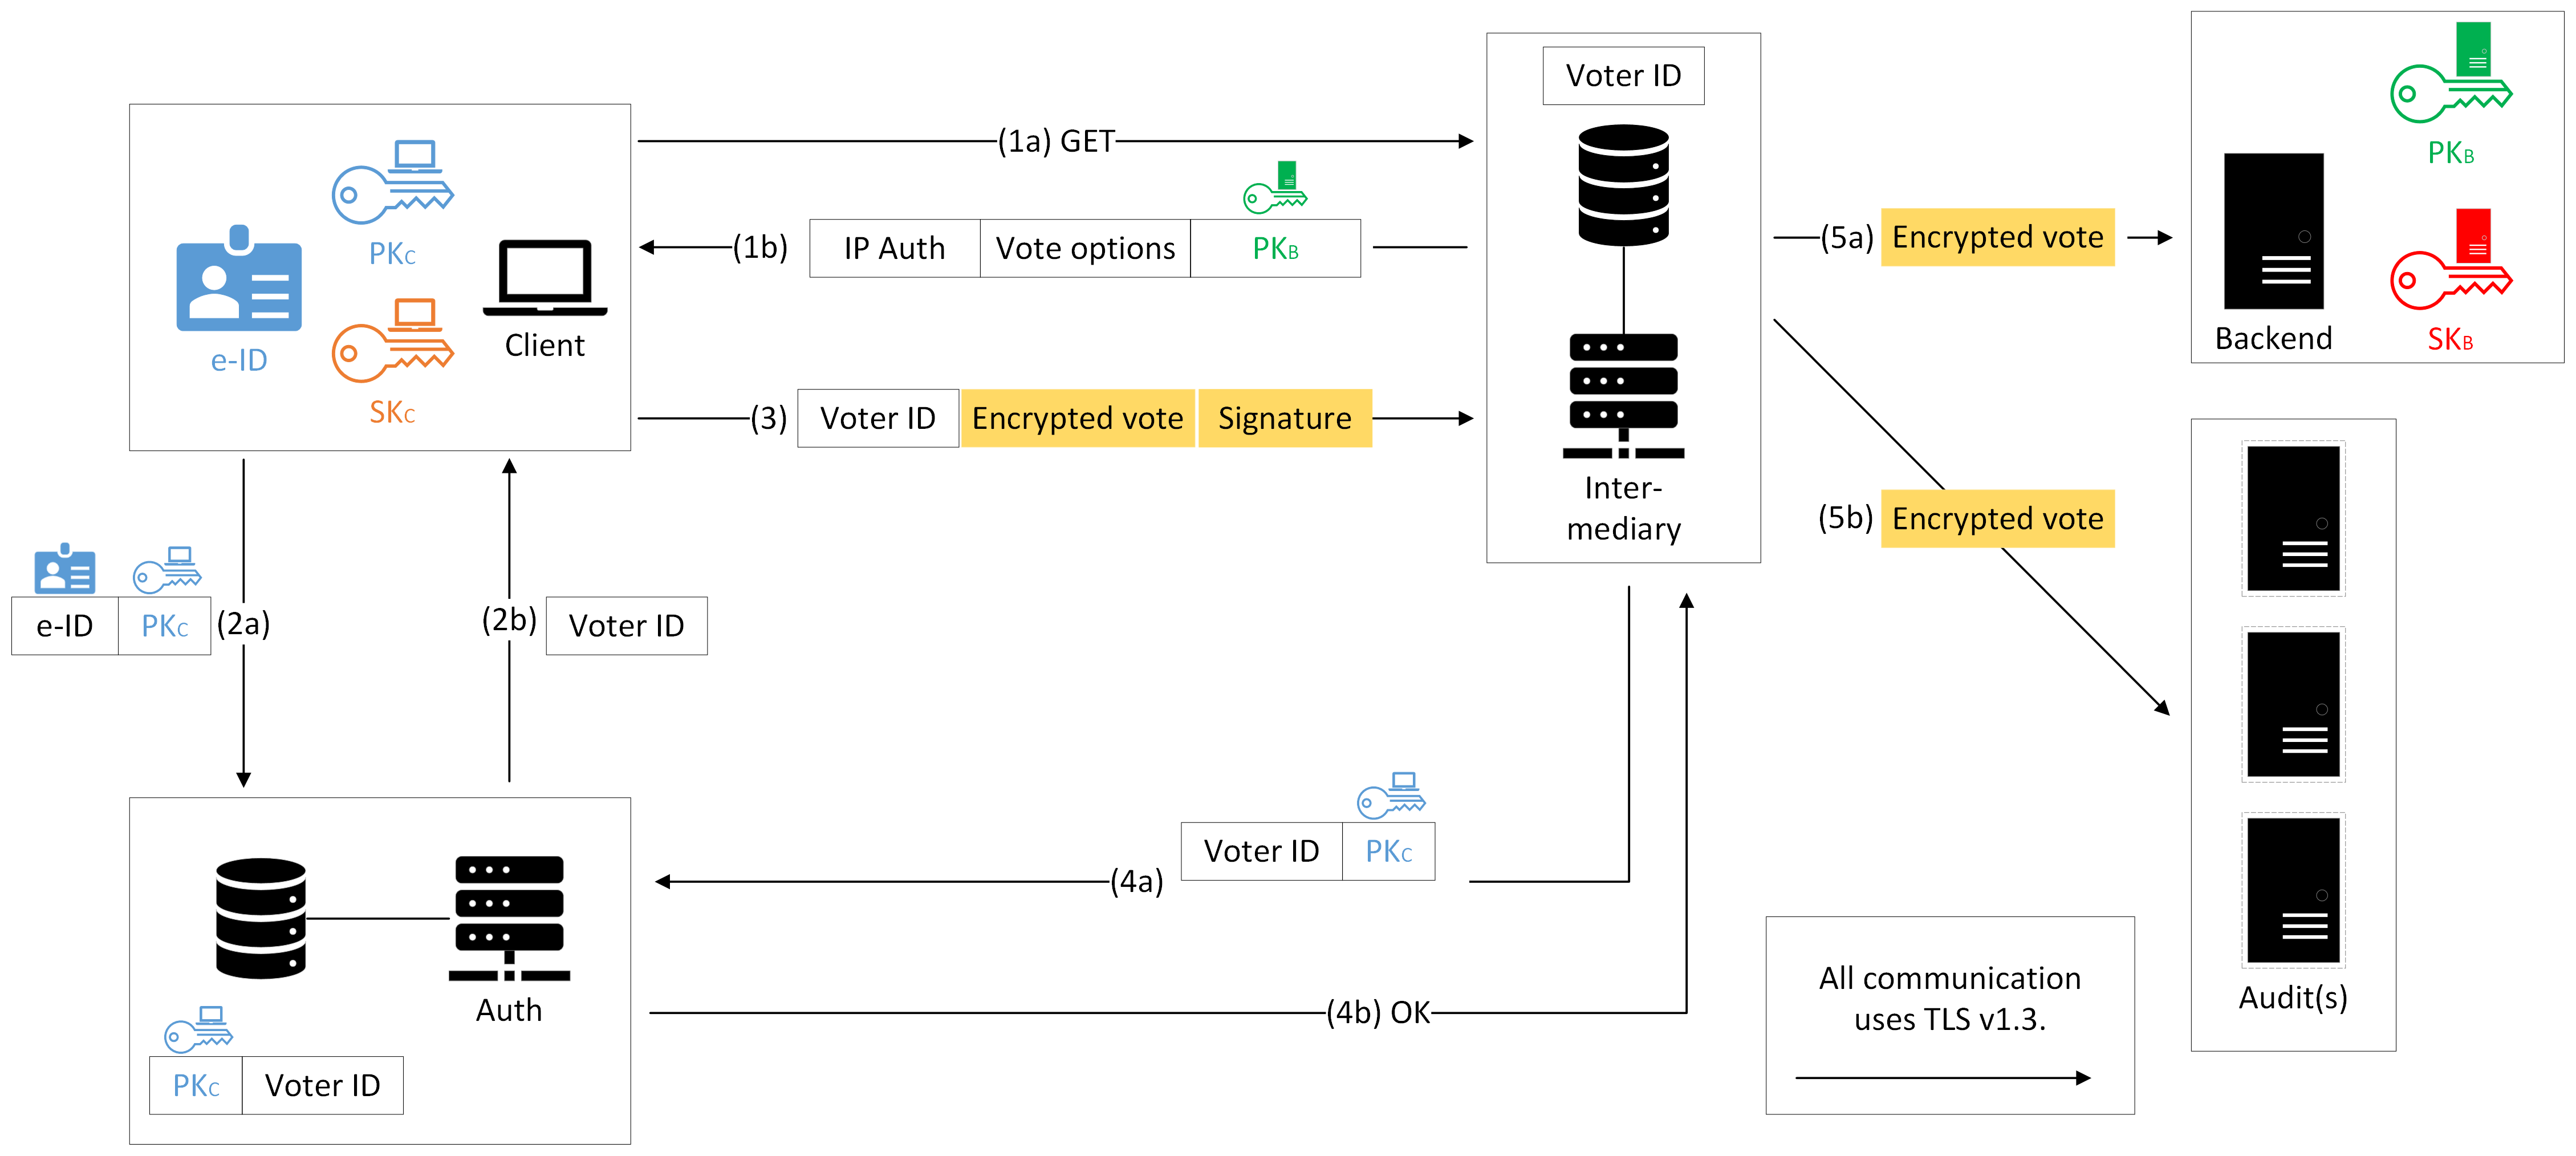
\includegraphics[width=\textwidth]{Schematic}
    \caption{The web-based model}\label{fig:schematic}
\end{figure}

\begin{figure}
    \centering
    \begin{subfigure}{0.48\textwidth}
        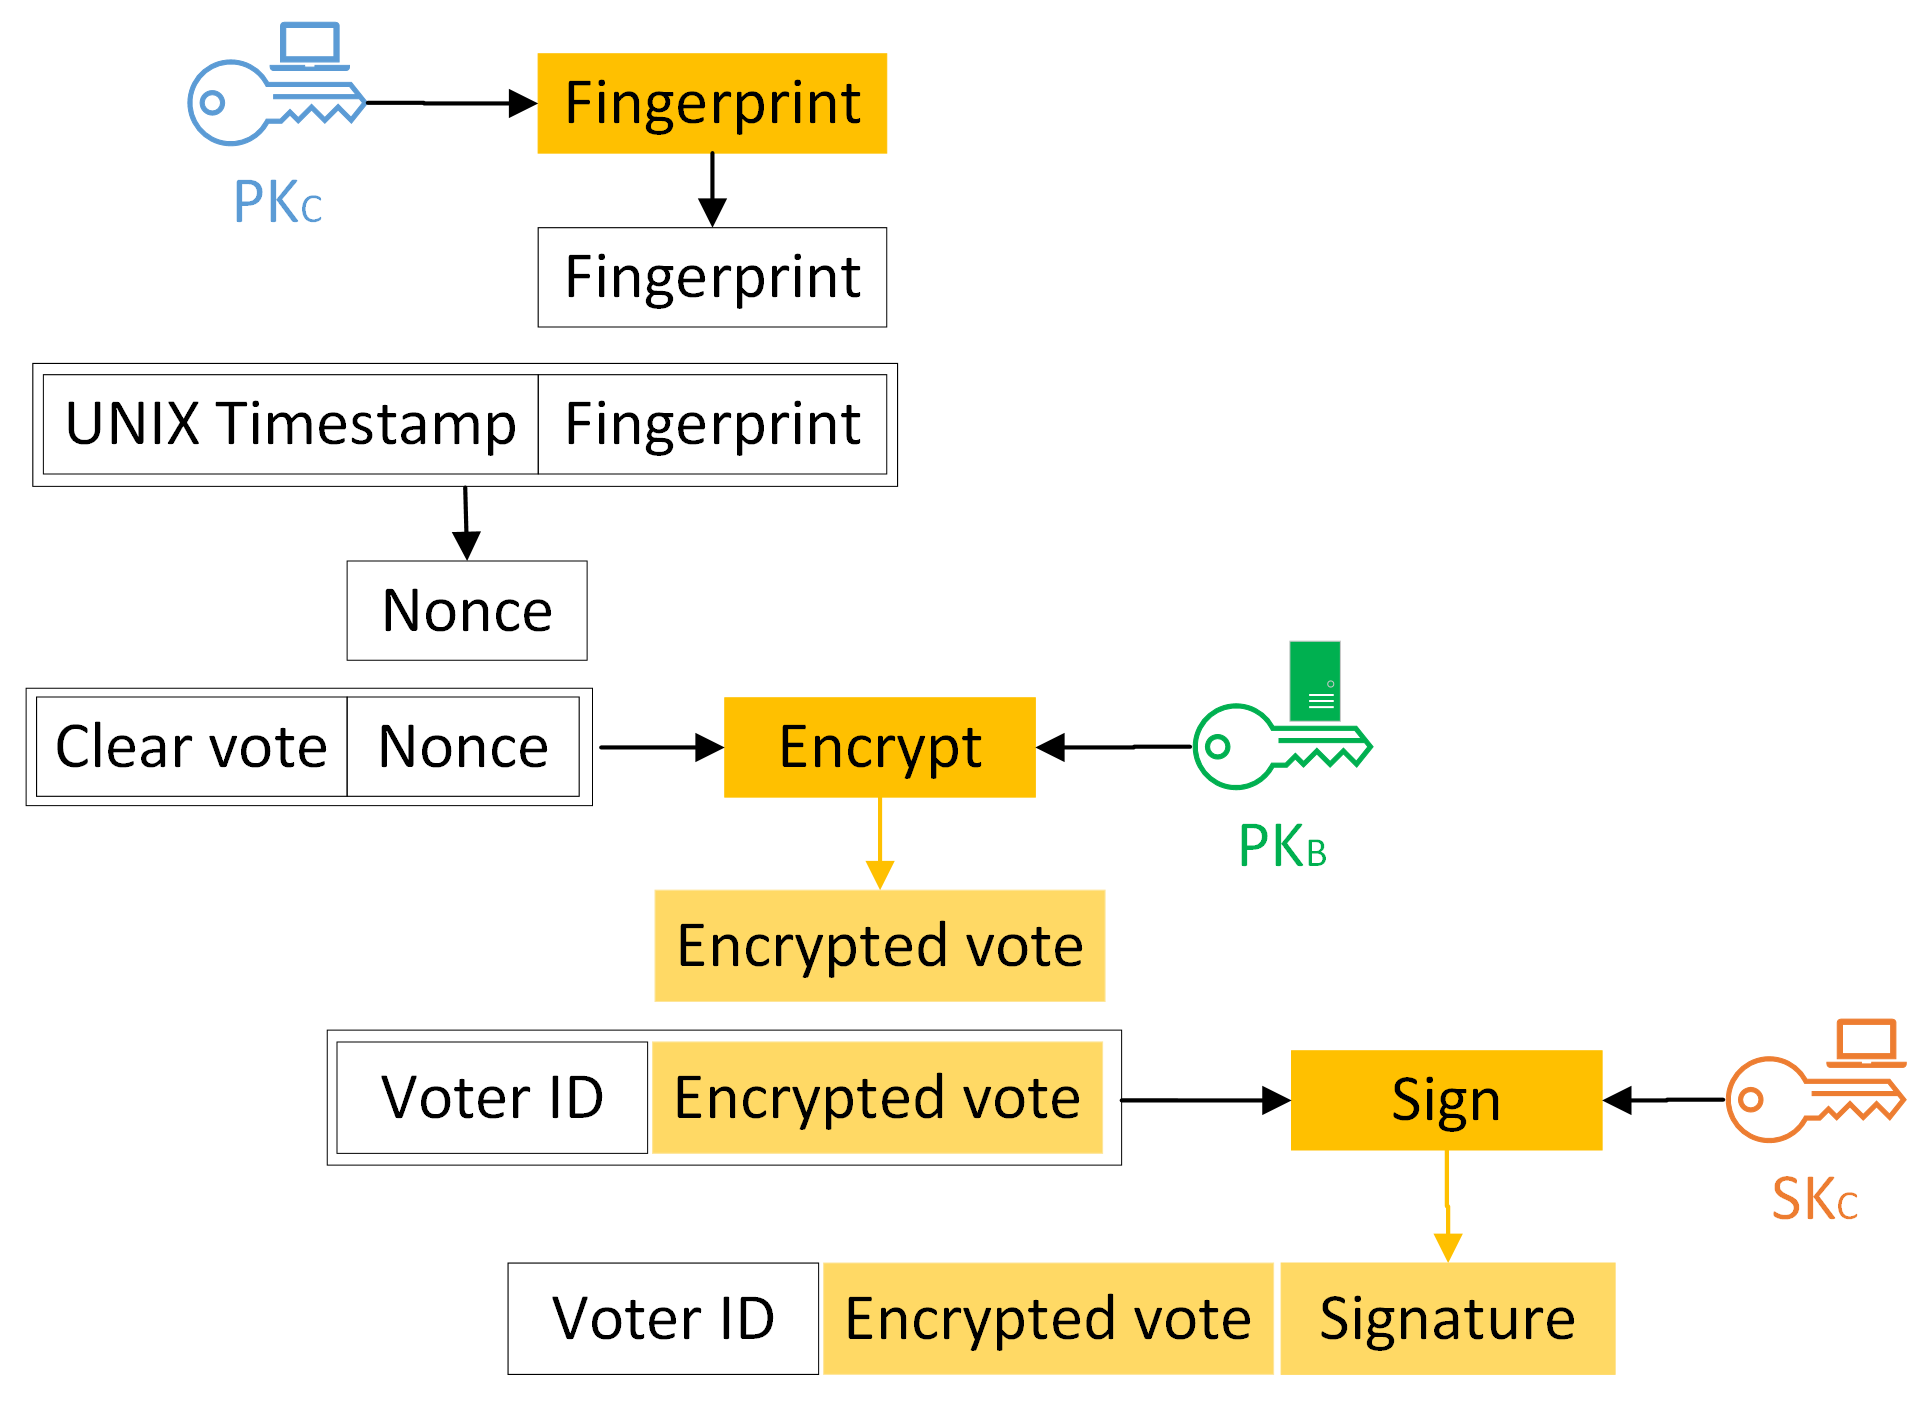
\includegraphics[width=\textwidth]{Client_Protocol}
        \caption{Client protocol}\label{fig:client}
    \end{subfigure}
    \begin{subfigure}{0.48\textwidth}
        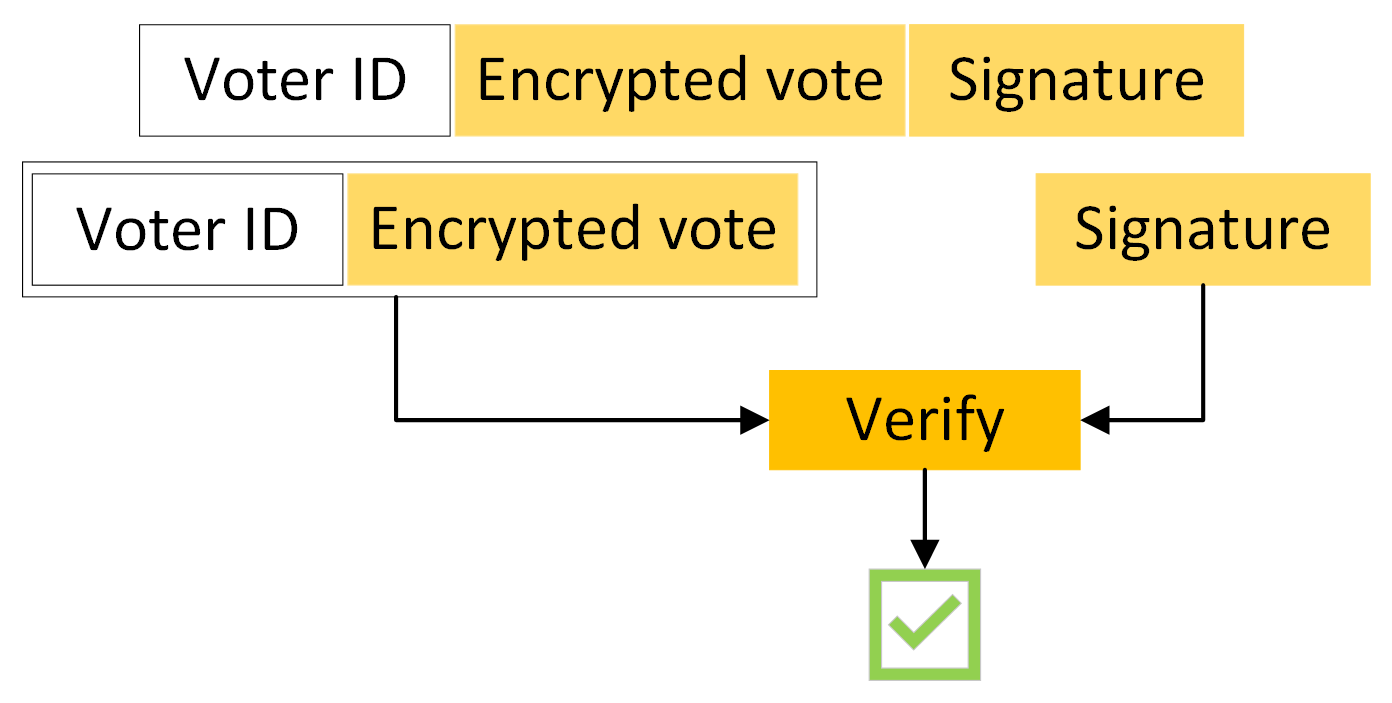
\includegraphics[width=\textwidth]{Intermediary_Protocol}
        \caption{Intermediary protocol}\label{fig:intermediary}
    \end{subfigure}
    \caption{Protocols in the web-based model}
\end{figure}

\begin{align}
    \text{Signed vote} &:= \text{Sig}_{SK_C}(\text{Enc}_{PK_B}(\text{vote}, \text{salt}), \text{voter ID})\label{formula:signed_vote}
\end{align}

Please use formula \ref{formula:signed_vote} to check whether.

\section{Attacks and their countermeasures}\label{sec:attacks}

\section{Limitations and vulnerabilities}\label{sec:limitations}

\section{Conclusion}\label{sec:conclusion}

\newpage

\printbibliography

\end{document}
